\clearpage
\section{维修站角色悬空}

在维修站按住 Ctrl，侧面可以看见靴子和地面之间留着一条缝。角色倒下以后，这条缝还在。更明显的一次出现在跳起时：玩家在空中受到电缆伤害，翻身动画一直播放，但动画播完，机器人还停在半空。下图保留了同一侧面机位。旧版这一次躺稳后，模型最低点距路面仍有 1.17 米。

\begin{center}
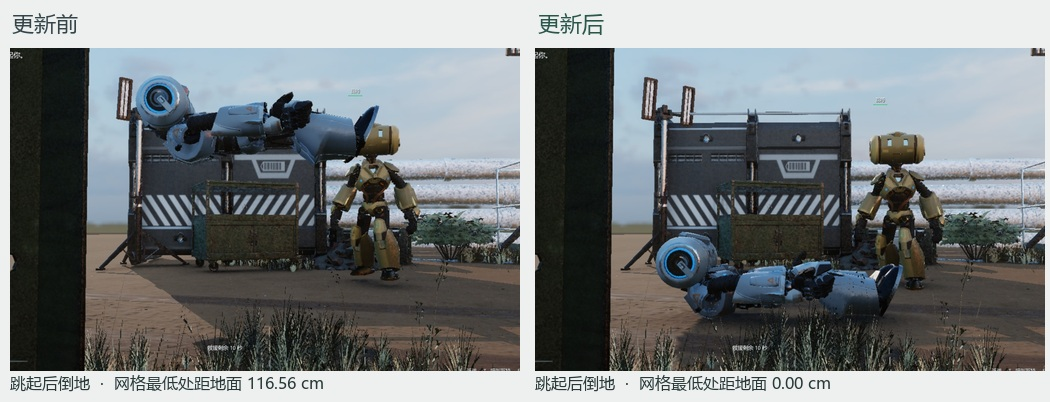
\includegraphics[width=\linewidth,height=.25\textheight,keepaspectratio]{../../../output/validation/packaged-watt/ground-contact/airborne.jpg}
\end{center}

\textbf{先量路面，再量角色。} 出生位置处可见的砂石平面高度是 $-0.025$ 米。旧关卡在它上方另放了一层不可见的盒形地板，盒顶高 $0.010$ 米。人物出生在 $0.080$ 米，移动代码又把第一次测得的脚下空隙保留到了后面每一步。两处相加，蹲伏时便留下了 $0.080-(-0.025)=0.105$ 米。我们另外播放了模型的蹲伏动作，量到支撑脚到模型地面的差最多约 0.15 毫米。动作自身不足以解释这十多厘米。

新版让砂石与碰撞地面共用同一高度。人物移动时从碰撞体的底部找支撑；这样既能使用原点在脚底的人物，也能使用原点在身体中央的人物。玩家和瓦特站立时用竖直的胶囊，蹲下时顶端下降，底端位置保持。倒下时，脚本读胸骨和骨盆的位置，等躯干接近水平，再把胶囊沿身体放平。背后的装甲包最先接触地面，胸甲下缘还高约 1.44 厘米，两只靴子也会自然翘起。

\textbf{空中倒地还涉及游戏更新。} 旧脚本在生命耗尽后直接返回，跳跃也随之停止。新版仍然把每帧的时间交给原先的跳跃，让角色落回已经选好的落脚处。下面是倒地更新中保留的移动调用。水平输入为零，空中经过的时间仍会增加。

\loc{SandboxProject/Source/StationMotion.cs}
\begin{Code}
Vector3 delta = Vector3.Zero;
// 已经起跳时继续下落，身体的宽度从角色碰撞体读取。
traversal = GameWorld.TraverseWithCollider(id, ref delta, seconds, TraversalInput.Walk);
\end{Code}

在最终发行包里重拍，玩家原地蹲伏、地面倒地、半空受伤后落地，以及瓦特倒地，四次稳定姿势的模型最低点与砂石的高度差在记录精度下均为零。测量使用运行时的骨骼位置和模型顶点，固定侧面机位用于看清缝隙，另保留原场景第三人称的蹲伏实拍。逐帧数值和前后录像见 \path{output/validation/packaged-watt/ground-contact/}。

\clearpage
\subsection*{在 Forge 中调整碰撞体}

在层级中选中角色，把「场景 Scene」的「碰撞体」设成「选中」，黄色轮廓便会画在角色身上。下图使用游戏中的 Operator 模型。测试时把右侧属性面板里的半径从 0.35 米调到 0.46 米，保存，关闭编辑器，再打开同一份场景，轮廓和数值都保留了修改。切到「全部」还能看到角色脚下的盒形地台，适合从侧面检查脚底和地面是否贴合。

\begin{center}
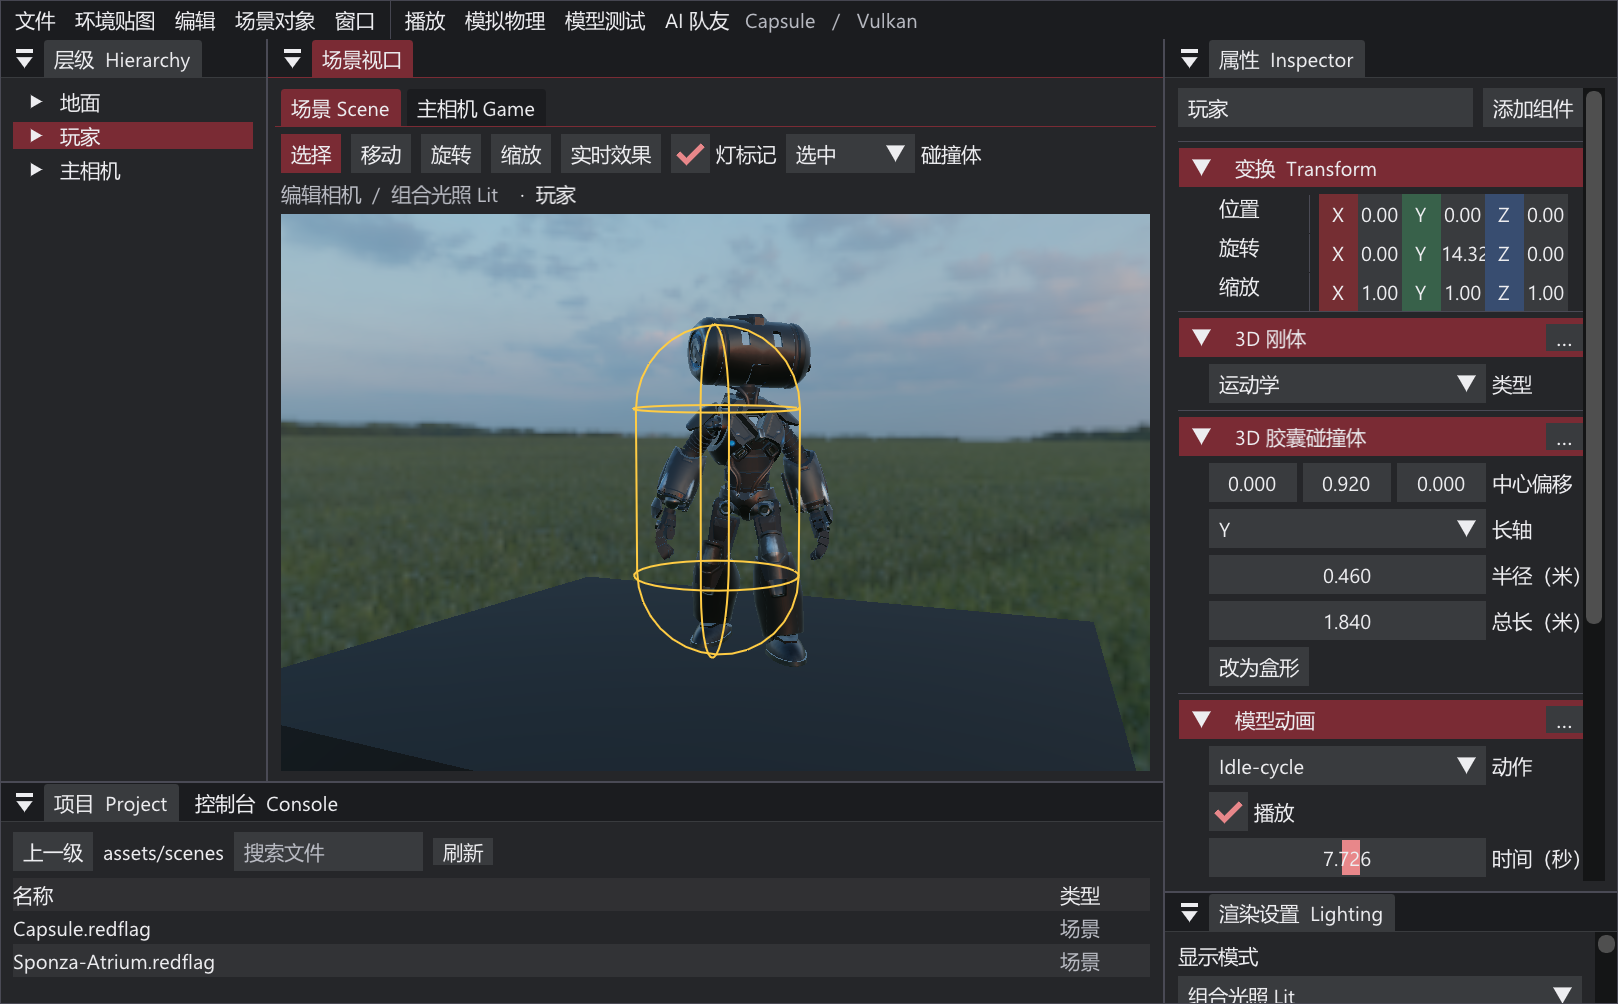
\includegraphics[width=\linewidth,height=.34\textheight,keepaspectratio]{../../../output/validation/packaged-watt/ground-contact/editor/reopened.png}
\end{center}

\textbf{刚体类型决定谁控制位置。} 维修棚的墙选静态（Static），在物理模拟中位置固定。一个要受重力落下的货箱可以选动态（Dynamic），由 PhysX 根据质量、受力和碰撞推进。维修员选运动学（Kinematic），脚本决定它要走多远，移动过程中用物理查询检查墙和落脚处。即使两件物品都用盒形，固定的墙和会落下的货箱仍然可以有完全不同的行为。

\textbf{碰撞体决定接触时使用的外形。} Forge 里的胶囊总长从一个圆头量到另一个圆头。以本关的站姿为例，总长 1.84 米、半径 0.35 米，中间直段长 $1.84-2\times0.35=1.14$ 米。PhysX 的参数是直段的半长，所以源码传入 0.57 米。胶囊沿本地 Y 轴放置时，它的底部正好落在角色原点，转向时身体宽度保持一致。

为检查半径会不会影响玩法，在同一面墙前按住 W，分别用 0.20 米和 0.52 米的角色半径走到不能再向前。角色原点最终距墙 0.181 米和 0.468 米。走路时引擎在胸部和头部各向前扫一个球，这两个球取角色半径的九成，所以停下时可以比黄色轮廓稍靠近墙。遇到静止角色时的射线查询使用完整的 PhysX 胶囊。

球形、平面、凸包、三角网格也是 PhysX 可用的几何形状。凸包可把不规则石块表面的顶点围成一个没有凹口的外壳。要让 Forge 作者使用它，项目还需要保存源网格引用，将顶点转换成 PhysX 的碰撞网格，并在视口中显示生成的外壳。当前 Forge 可编辑的 3D 碰撞组件包括盒形和胶囊，地形组件可从高度图生成物理表面。球形扫掠已经用于镜头避障。

\loc{Redflag/src/Redflag/Physics/PhysicsWorld.cpp}
\note{参考：NVIDIA PhysX 5.6.1 文档，\href{https://nvidia-omniverse.github.io/PhysX/physx/5.6.1/docs/RigidBodyOverview.html}{Rigid Body Overview} 与 \href{https://nvidia-omniverse.github.io/PhysX/physx/5.6.1/docs/Geometry.html}{Geometry}。}
